\documentclass{standalone}

\usepackage{hyperref}
\usepackage{tikz}

\usetikzlibrary{decorations.pathreplacing,
  arrows,
  calc,
  decorations.pathmorphing,
  decorations.pathreplacing,
  decorations.markings,
  positioning,
  shapes,
  3d
}

\tikzstyle{snakearrow} = [decorate, decoration={pre length=0.2cm,
  post length=0.2cm, snake, amplitude=.4mm,
  segment length=2mm},thick, ->]

\ifpdf
% Ensure reproducible output
\pdfinfoomitdate=1
\pdfsuppressptexinfo=-1
\pdftrailerid{}
\hypersetup{
  pdfcreator={},
  pdfproducer={}
}
\fi

\begin{document}
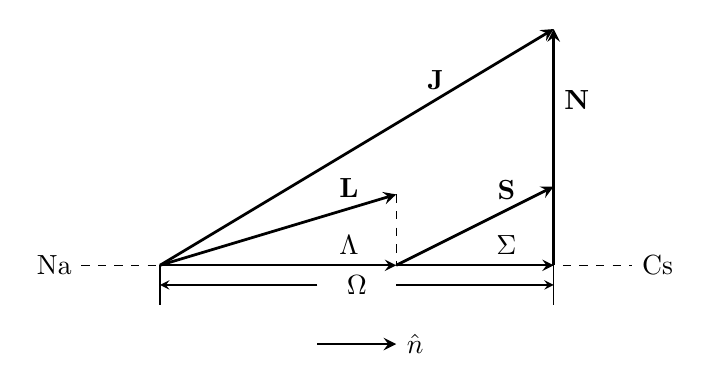
\begin{tikzpicture}
  \draw[->,>=stealth,line width=1] (-0.5, -1) -- (0.5, -1) node[right] {$\hat{n}$};
  \draw[dashed] (-3.5, 0) node[left] {Na} -- (3.5, 0) node[right] {Cs};

  % Lambda
  \draw[->,>=stealth,line width=0.8] (-2.5, 0) -- node[above,pos=0.8] {$\Lambda$} (0.5, 0);
  \draw[->,>=stealth,line width=1] (-2.5, 0) -- node[above,pos=0.8] {$\mathbf{L}$} (0.5, 0.9);
  \draw[dashed] (0.5, 0.9) -- (0.5, 0);

  % Sigma
  \draw[->,>=stealth,line width=0.8] (0.5, 0) -- node[above,pos=0.7] {$\Sigma$} (2.5, 0);
  \draw[->,>=stealth,line width=1] (0.5, 0) -- node[above,pos=0.7] {$\mathbf{S}$} (2.5, 1);

  % Omega
  \draw (-2.5, 0) -- (-2.5, -0.5);
  \draw (2.5, 0) -- (2.5, -0.5);
  \draw[->,>=stealth,line width=0.5] (-0.5, -0.25) -- (-2.5, -0.25);
  \draw[->,>=stealth,line width=0.5] (0.5, -0.25) -- (2.5, -0.25);
  \node at (0, -0.25) {$\Omega$};

  % J
  \draw[->,>=stealth,line width=1] (-2.5, 0) -- node[above,pos=0.7] {$\mathbf{J}$} (2.5, 3);
  \draw[->,>=stealth,line width=1] (2.5, 0) -- node[right,pos=0.7] {$\mathbf{N}$} (2.5, 3);
\end{tikzpicture}
\end{document}
